% Options for packages loaded elsewhere
\PassOptionsToPackage{unicode}{hyperref}
\PassOptionsToPackage{hyphens}{url}
%
\documentclass[
  a4paperpaper,
]{article}
\usepackage{lmodern}
\usepackage{amssymb,amsmath}
\usepackage{ifxetex,ifluatex}
\ifnum 0\ifxetex 1\fi\ifluatex 1\fi=0 % if pdftex
  \usepackage[T1]{fontenc}
  \usepackage[utf8]{inputenc}
  \usepackage{textcomp} % provide euro and other symbols
\else % if luatex or xetex
  \usepackage{unicode-math}
  \defaultfontfeatures{Scale=MatchLowercase}
  \defaultfontfeatures[\rmfamily]{Ligatures=TeX,Scale=1}
\fi
% Use upquote if available, for straight quotes in verbatim environments
\IfFileExists{upquote.sty}{\usepackage{upquote}}{}
\IfFileExists{microtype.sty}{% use microtype if available
  \usepackage[]{microtype}
  \UseMicrotypeSet[protrusion]{basicmath} % disable protrusion for tt fonts
}{}
\makeatletter
\@ifundefined{KOMAClassName}{% if non-KOMA class
  \IfFileExists{parskip.sty}{%
    \usepackage{parskip}
  }{% else
    \setlength{\parindent}{0pt}
    \setlength{\parskip}{6pt plus 2pt minus 1pt}}
}{% if KOMA class
  \KOMAoptions{parskip=half}}
\makeatother
\usepackage{xcolor}
\IfFileExists{xurl.sty}{\usepackage{xurl}}{} % add URL line breaks if available
\IfFileExists{bookmark.sty}{\usepackage{bookmark}}{\usepackage{hyperref}}
\hypersetup{
  pdftitle={爬山演算法},
  pdfauthor={陳鍾誠},
  hidelinks,
  pdfcreator={LaTeX via pandoc}}
\urlstyle{same} % disable monospaced font for URLs
\usepackage{color}
\usepackage{fancyvrb}
\newcommand{\VerbBar}{|}
\newcommand{\VERB}{\Verb[commandchars=\\\{\}]}
\DefineVerbatimEnvironment{Highlighting}{Verbatim}{commandchars=\\\{\}}
% Add ',fontsize=\small' for more characters per line
\newenvironment{Shaded}{}{}
\newcommand{\AlertTok}[1]{\textcolor[rgb]{1.00,0.00,0.00}{\textbf{#1}}}
\newcommand{\AnnotationTok}[1]{\textcolor[rgb]{0.38,0.63,0.69}{\textbf{\textit{#1}}}}
\newcommand{\AttributeTok}[1]{\textcolor[rgb]{0.49,0.56,0.16}{#1}}
\newcommand{\BaseNTok}[1]{\textcolor[rgb]{0.25,0.63,0.44}{#1}}
\newcommand{\BuiltInTok}[1]{#1}
\newcommand{\CharTok}[1]{\textcolor[rgb]{0.25,0.44,0.63}{#1}}
\newcommand{\CommentTok}[1]{\textcolor[rgb]{0.38,0.63,0.69}{\textit{#1}}}
\newcommand{\CommentVarTok}[1]{\textcolor[rgb]{0.38,0.63,0.69}{\textbf{\textit{#1}}}}
\newcommand{\ConstantTok}[1]{\textcolor[rgb]{0.53,0.00,0.00}{#1}}
\newcommand{\ControlFlowTok}[1]{\textcolor[rgb]{0.00,0.44,0.13}{\textbf{#1}}}
\newcommand{\DataTypeTok}[1]{\textcolor[rgb]{0.56,0.13,0.00}{#1}}
\newcommand{\DecValTok}[1]{\textcolor[rgb]{0.25,0.63,0.44}{#1}}
\newcommand{\DocumentationTok}[1]{\textcolor[rgb]{0.73,0.13,0.13}{\textit{#1}}}
\newcommand{\ErrorTok}[1]{\textcolor[rgb]{1.00,0.00,0.00}{\textbf{#1}}}
\newcommand{\ExtensionTok}[1]{#1}
\newcommand{\FloatTok}[1]{\textcolor[rgb]{0.25,0.63,0.44}{#1}}
\newcommand{\FunctionTok}[1]{\textcolor[rgb]{0.02,0.16,0.49}{#1}}
\newcommand{\ImportTok}[1]{#1}
\newcommand{\InformationTok}[1]{\textcolor[rgb]{0.38,0.63,0.69}{\textbf{\textit{#1}}}}
\newcommand{\KeywordTok}[1]{\textcolor[rgb]{0.00,0.44,0.13}{\textbf{#1}}}
\newcommand{\NormalTok}[1]{#1}
\newcommand{\OperatorTok}[1]{\textcolor[rgb]{0.40,0.40,0.40}{#1}}
\newcommand{\OtherTok}[1]{\textcolor[rgb]{0.00,0.44,0.13}{#1}}
\newcommand{\PreprocessorTok}[1]{\textcolor[rgb]{0.74,0.48,0.00}{#1}}
\newcommand{\RegionMarkerTok}[1]{#1}
\newcommand{\SpecialCharTok}[1]{\textcolor[rgb]{0.25,0.44,0.63}{#1}}
\newcommand{\SpecialStringTok}[1]{\textcolor[rgb]{0.73,0.40,0.53}{#1}}
\newcommand{\StringTok}[1]{\textcolor[rgb]{0.25,0.44,0.63}{#1}}
\newcommand{\VariableTok}[1]{\textcolor[rgb]{0.10,0.09,0.49}{#1}}
\newcommand{\VerbatimStringTok}[1]{\textcolor[rgb]{0.25,0.44,0.63}{#1}}
\newcommand{\WarningTok}[1]{\textcolor[rgb]{0.38,0.63,0.69}{\textbf{\textit{#1}}}}
\usepackage{longtable,booktabs}
% Correct order of tables after \paragraph or \subparagraph
\usepackage{etoolbox}
\makeatletter
\patchcmd\longtable{\par}{\if@noskipsec\mbox{}\fi\par}{}{}
\makeatother
% Allow footnotes in longtable head/foot
\IfFileExists{footnotehyper.sty}{\usepackage{footnotehyper}}{\usepackage{footnote}}
\makesavenoteenv{longtable}
\usepackage{graphicx,grffile}
\makeatletter
\def\maxwidth{\ifdim\Gin@nat@width>\linewidth\linewidth\else\Gin@nat@width\fi}
\def\maxheight{\ifdim\Gin@nat@height>\textheight\textheight\else\Gin@nat@height\fi}
\makeatother
% Scale images if necessary, so that they will not overflow the page
% margins by default, and it is still possible to overwrite the defaults
% using explicit options in \includegraphics[width, height, ...]{}
\setkeys{Gin}{width=\maxwidth,height=\maxheight,keepaspectratio}
% Set default figure placement to htbp
\makeatletter
\def\fps@figure{htbp}
\makeatother
\setlength{\emergencystretch}{3em} % prevent overfull lines
\providecommand{\tightlist}{%
  \setlength{\itemsep}{0pt}\setlength{\parskip}{0pt}}
\setcounter{secnumdepth}{-\maxdimen} % remove section numbering

\title{爬山演算法}
\author{陳鍾誠}
\date{2019 年 6 月 5 日}

\begin{document}
\maketitle

\hypertarget{ux6458ux8981}{%
\subsection{摘要}\label{ux6458ux8981}}

爬山演算法 (Hill Climbing)
是一種最簡單的優化算法,該方法就像模擬人類爬山時的行為而設計的,因此稱為爬山演算法。

\hypertarget{ux7c21ux4ecb}{%
\subsection{簡介}\label{ux7c21ux4ecb}}

以下是「爬山演算法」 (Hill-Climbing Algorithm)
的一個簡易版本,其方法超簡單,就是一直看旁邊有沒有更好的解,如果有就移過去。然後反覆的作這樣的動作,直到旁邊的解都比現在的更差時,程式就停止,然後將那個位於山頂的解傳回,就完成了。

\begin{Shaded}
\begin{Highlighting}[]
\NormalTok{Algorithm }\AttributeTok{HillClimbing}\NormalTok{(f}\OperatorTok{,}\NormalTok{ x)}
\NormalTok{  x }\OperatorTok{=}\NormalTok{ 隨意設定一個解。}
  \ControlFlowTok{while}\NormalTok{ (x 有鄰居 x}\StringTok{' 比 x 更高)}
\NormalTok{    x }\OperatorTok{=}\NormalTok{ x}\StringTok{';}
\NormalTok{  end}
  \ControlFlowTok{return}\NormalTok{ x}\OperatorTok{;}
\NormalTok{end}
\end{Highlighting}
\end{Shaded}

當然、這種演算法只能找到「局部最佳解」(local
optimal),當整個空間有很多山頂的時候,這種方法會爬到其中一個山頂就停了,並不一定會爬到最高的山頂。

\hypertarget{ux6587ux737bux56deux9867}{%
\subsection{文獻回顧}\label{ux6587ux737bux56deux9867}}

必須引用 (Pizza et al. (2000)) 才會出現在最後的 Reference 裏。

\hypertarget{ux5716ux7247}{%
\subsection{圖片}\label{ux5716ux7247}}

程式究竟要怎麼爬山呢?且讓我們用一張圖來看看。假如我們在 Google
裏輸入一個算式,Google 會幫我們畫出該函數。舉例而言,如果我在 Google
輸入 \(x^2+3x+5\) 這個算式,您會看到如 \protect\hyperlink{image1}{圖1}
所示的結果。

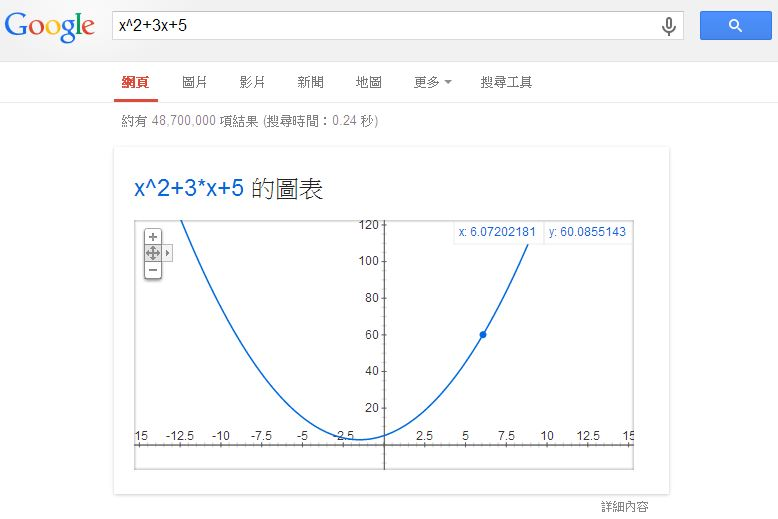
\includegraphics{img/GoogleGraph2D.jpg}

\hypertarget{ux8868ux683c}{%
\subsection{表格}\label{ux8868ux683c}}

\hypertarget{tables}{%
\subsection{Tables}\label{tables}}

Table 1: Example Markdown table

\begin{longtable}[]{@{}ll@{}}
\toprule
欄位 & 內容\tabularnewline
\midrule
\endhead
\href{https://www.cakeresume.com/f5611f}{履歷} & to
\href{cccForStudent.md}{學生} , \href{cccForProgrammer.md}{程式人} ,
\href{cccForProfessor.md}{教授} ,
\href{cccForCompany.md}{公司}\tabularnewline
職務 & \href{http://www.nqu.edu.tw/}{金門大學} /
\href{http://www.nqu.edu.tw/educsie/index.php}{資訊工程} /
\href{http://www.nqu.edu.tw/educsie/index.php?act=blog\&code=list\&ids=4}{教師}\tabularnewline
專長 & 寫程式 ( \href{https://nodejs.org/}{NodeJS} +
\href{js1.md}{JavaScript} + \href{c1.md}{C} ) , 寫書 (
\href{https://zh.wikipedia.org/wiki/Markdown}{Markdown} )\tabularnewline
聯絡 & ccckmit@gmail.com ,
\href{https://www.facebook.com/ccckmit}{Facebook}\tabularnewline
帳號 & \href{https://github.com/ccckmit}{Github} ,
\href{http://www.slideshare.net/ccckmit/}{SlideShare} ,
\href{https://www.youtube.com/user/ccckmit}{YouTube}\tabularnewline
作品 & \href{course.md}{課程} , \href{booklist.md}{書籍} ,
\href{codelist.md}{程式} , \href{novel.md}{小說} ,
\href{article.md}{散文} , \href{../poem/}{詩} , \href{../slide/}{十
分鐘系列}\tabularnewline
研究 & \href{../bot/}{聊天機器人} , \href{../mt/}{機器翻譯} ,
\href{../artilang/}{人造語} , \href{../mdo/}{Markdown
物件格式應用}\tabularnewline
關注 & \href{tool.md}{軟體工具} , \href{topic.md}{研究主題} ,
\href{language.md}{程式語言} ,
\href{turingAward.md}{圖靈獎}\tabularnewline
\bottomrule
\end{longtable}

\hypertarget{ux6f14ux7b97ux6cd5}{%
\subsection{演算法}\label{ux6f14ux7b97ux6cd5}}

數學式

\[
\int_0^x f(x) dx
\]

嵌入式 : \(\sum_{i=1}^n p(i) \log \; p(i)\)

\[
\frac{p(i) log p(i)}{\sqrt{n}}
\]

\[
\frac{-b \pm \sqrt{b^2-4ac}}{2a}
\]

\hypertarget{ux53c3ux8003ux6587ux737b}{%
\subsection*{參考文獻}\label{ux53c3ux8003ux6587ux737b}}
\addcontentsline{toc}{subsection}{參考文獻}

\hypertarget{refs}{}
\leavevmode\hypertarget{ref-pizza2000identification}{}%
Pizza, Mariagrazia, Vincenzo Scarlato, Vega Masignani, Marzia Monica
Giuliani, Beatrice Arico, Maurizio Comanducci, Gary T Jennings, et al.
2000. ``Identification of Vaccine Candidates Against Serogroup B
Meningococcus by Whole-Genome Sequencing.'' \emph{Science} 287 (5459):
1816--20.

\end{document}
